\chapter{Analitična izpeljava vplivov dinamične in statične ekscentričnosti}

V tem poglavju je analitično izpeljan vpliv ekscentričnosti, ki se pojavita zaradi neprimerne vgradnje. Napaki različno vplivati na izhodni podatek, zato se ju lahko obravna posamično. Preko analitične izpeljave je prikazano, kako se spreminja lokacija Hall-ove sonde glede na magnet ob pravilni montaži. Z vpeljavo dodatne ekscentričnosti v model se potek gibanja sonde glede na magnet spremeni. S poznavanjem lokacije sonde nad magnetom se lahko odčita pomerjena vrednost \Bz.


\section{Definicija koordinatnih sistemov}

Definiran kartezični koordinatni sistem, ima v izhodišcu postavljen radialno magnetiziran magnet. Na poljubno točko $S_{h0}(x_0,y_0)$, vendar ne v izhodišče je postavljena Hall-ova sonda (slika \ref{fig:def_kks}). Za lažjo predstavo se Hall-ova sonda nahaja na abcisno osi.

\begin{figure}[h!]
	\centering
	\begin{tikzpicture}
	\magnet {0} {0} {0}{$S_r(0, 0)$}{1};
	\hall {2.3}{0} {0};
	\end{tikzpicture}
	\caption{Definicija koordinatnega sistema z magnetom in Hall-ovo sondo}
	\label{fig:def_kks}
\end{figure}

Z rotacijo magneta za kot $\theta$, se položa sonde glede na magnet spremeni. Nov položaj sonde glede na magnet je enaka, če namesto magnet, zavrtimo sondo za kot $-\theta$ . Nov položaj sonde glede na magnet lahko zapišemo z (\ref{equ:rotacija_hall}).

\begin{equation}
\label{equ:rotacija_hall}
\begin{bmatrix} x\\y \end{bmatrix}=
\begin{bmatrix} \cos(-\theta)&-\sin(-\theta)\\\sin(-\theta)&\cos(-\theta) \end{bmatrix}
\begin{bmatrix} x_0\\y_0 \end{bmatrix}
\end{equation}

Argument rotacijske matrike je $-\theta$. Z upoštevanjem lihosti funkcije sinus in sodosti funkcije kosinus\cite{Matematika1}, se (\ref{equ:rotacija_hall}) poenostavi v:
\begin{equation}
\label{equ:rotacija_hall_simplify}
\begin{bmatrix} x\\y \end{bmatrix}=
\begin{bmatrix} \cos(\theta)&\sin(\theta)\\-\sin(\theta)&\cos(\theta) \end{bmatrix}
\begin{bmatrix} x_0\\y_0 \end{bmatrix}
\end{equation}




\begin{figure}[h!]
%	\centering


    \begin{subfigure}[b]{0.5\textwidth}
	\centering
	
		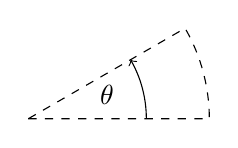
\begin{tikzpicture}
		[scale=1, every node/.style={scale=1}]
				\magnet {0} {0} {30}{}{1}
				\hall {2.3}{0} {0};
				\draw [dashed](0,0)--(2.3,0) arc (0:30:2.3)--(0,0);
				\node at(1,0.3){$\theta$};
                \draw [->] (1.5,0) arc (0:30:1.5);
		\end{tikzpicture}
	\caption{Zasukan magnet za kot $\mathrm{\theta}$}
	\label{subfig:zasuk_magnet}
\end{subfigure}
\begin{subfigure}[b]{0.5\textwidth}
	\centering
	
		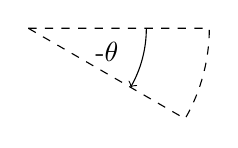
\begin{tikzpicture}[scale=1, every node/.style={scale=1}]		
				\magnet {0} {0} {0}{}{1}
				\hall {1.99}{-1.15} {-30};
				\draw [dashed](0,0)--(2.3,0) arc (0:-30:2.3)--(0,0);
				\node at(1,-0.3){-$\theta$};
                \draw [->] (1.5,0) arc (0:-30:1.5);
		\end{tikzpicture}
	
	\caption{Zasukan senzor za kot $\mathrm{-\theta}$}
	\label{subfig:zasuk_hall}
\end{subfigure}

\caption{Sprememba položaja glede na magnet ob rotaciji}
\label{fig:zasuk_magneta}

\end{figure}



\section{Izpeljava gibanja položaja Hallove sonde na magnet pri dinamični ekscentričnosti}

Magnet je postavljen v izhodišce koordinatnega sistema $S_m(0,0)$, kjer je os vrtenja. Vpliv dinamične ekscentričnosti je sprememba središča magneta v točko $S_{m1}(\Delta x_d,\Delta y_d)$ (Slika \ref{fig:def_din_eks}). Os vrtenja je ostaja v izhodišču koordinatnega sistema. Središce magneta $S_{m1}(\Delta x_d,\Delta y_d)$ ob rotaciji opiše okoli osi vrtenja krožnico z radijem $\sqrt{\Delta x_d^2+\Delta y_d^2}$.

\begin{figure}[h!]
	\centering
	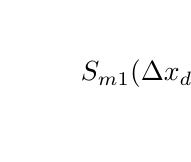
\begin{tikzpicture}
		\magnet {0.6} {0.3} {0}{$S_{m1}(\Delta x_d,\Delta y_d)$}{1};
		\draw [dashed]  (0,0) circle (0.67);
		\draw (0,0)--(0.6,0.3);
		\fill (0,0) circle [radius=1pt];
		\node at (0.35,-0.3){$S_0(0,0)$};
		\hall {2.3}{0} {0};
		\kks{3}
	\end{tikzpicture}
	\caption{Definicije dinamične ekscentričnosti}
	\label{fig:def_din_eks}
\end{figure}

\begin{equation}
\label{equ:rotacija_hall_din_sonda}
\begin{bmatrix} x\\y \end{bmatrix}=
\begin{bmatrix} x_0\\y_0 \end{bmatrix}+
\begin{bmatrix} \cos(\theta)&\sin(\theta)\\-\sin(\theta)&\cos(\theta) \end{bmatrix}\cdot
\begin{bmatrix} x_d\\y_d \end{bmatrix}
\end{equation}
S (\ref{equ:rotacija_hall_din_sonda}) je izraženo gibanje središče magneta na Hallovo sondo. Celoten sistem se vrti okoli osi vrtenja $S_0(0,0)$. Velja enak razmislek kot v prejšnjem poglavju z vrtenjem sonde za kot  $-\theta$:
 
\begin{equation}
\label{equ:rotacija_hall_din_1}
\begin{bmatrix} x\\y \end{bmatrix}=
\begin{bmatrix} \cos(\theta)&-\sin(\theta)\\ \sin(\theta)&\cos(\theta) \end{bmatrix}
\cdot \begin{pmatrix}
\begin{bmatrix} x_0\\y_0 \end{bmatrix}+
\begin{bmatrix} \cos(\theta)&\sin(\theta)\\-\sin(\theta)&\cos(\theta) \end{bmatrix}\cdot
\begin{bmatrix} x_d\\y_d \end{bmatrix}\end{pmatrix}
\end{equation}

(\ref{equ:rotacija_hall_din_1}) se poenostavi:
\begin{equation}
\label{equ:rotacija_hall_din}
\begin{bmatrix} x\\y \end{bmatrix}=
\begin{bmatrix} \cos(\theta)&\sin(\theta)\\-\sin(\theta)&\cos(\theta) \end{bmatrix}
\begin{bmatrix} x_0\\y_0 \end{bmatrix}
-
\begin{bmatrix} \Delta x_d\\\Delta y_d \end{bmatrix}
\end{equation}

Dinamična ekscentričnost na gibanje sonde vpliva kot enosmerna komponenta  $(-\Delta x_d,-\Delta y_d)$. Enak učinek se doseže, z izmikom Hallove sonde in osi vrtenja v novo točko $S_{h1}(-\Delta x_d,-\Delta y_d), S_0(x_0-\Delta x_d,y_0-\Delta y_d)$  in zavrti sondo okoli osi vrtenja za  $-\theta$. 


%
%\begin{figure}[h!]
%	\centering
%	\begin{tikzpicture}
%		\magnet {0} {0} {0}{$S_{m}(0,0)$}{1};
%		\draw (0,0)--(-0.6,-0.3);
%		\fill (-0.6,-0.3) circle [radius=1pt];
%		\node at (0,-0.6){$S_0(-\Delta x_d,-\Delta y_d)$};
%		\hall {1.7}{-0.3} {0};
%		\kks{3}
%	\end{tikzpicture}
%	\caption{Shema definicije dinamične ekscentričnosti vpliva na Hall-ovo sondo}
%	\label{fig:def_din_eks_na_stator}
%\end{figure}
%
%Sistema prikazana na slikah \ref{fig:def_din_eks} in \ref{fig:def_din_eks_na_stator}, se v začetnih legah ne razlikujeta. Sedaj zarotirajmo Hall-ovo sondo okoli osi vrtenja $S_0(-\Delta x_d,-\Delta y_d)$. Hall-ova sonda se giblje glede na magnet enako, kot če bi magnet zavrteli z dinamično ekscentričnostjo (Slika \ref{fig:def_din_eks}). Gibanje Hall-ove sonde na magnet je izraženo kot gibanje po krožnici s središčem v točki $(-\Delta x_d,-\Delta y_d)$.
%
%\begin{figure}[h!]
%	\centering
%	\begin{tikzpicture}
%		\magnet {0} {0} {0}{}{1};
%		\draw [dotted]  (-0.6,-0.3) circle (2.3);
%		\draw (0,0)--(-0.6,-0.3);
%		\fill (-0.6,-0.3) circle [radius=1pt];
%		\hall {1.39}{-1.45} {-30};
%		\draw [dashed](-0.6,-0.3)--(1.7,-0.3) arc(0:-30:2.3)--(-0.6,-0.3);
%		\node at(0.4,-0.6){$-\theta$};
%        \draw [->] (0.9,-0.3) arc (0:-30:1.5);
%		\kks{3}
%	\end{tikzpicture}
%	\caption{Potek Hall-ove sonde ob rotaciji glede na magnet ob dinamični ekscentričnosti}
%	\label{fig:potek_sonde_din_eks}
%\end{figure}
%
%Potek Hall-ove sonde ob rotaciji z upoštevanjem dinamične ekscentričnosti lahko zapišemo kot rotacijo z dodatno enosmerno komponento(\ref{equ:rotacija_hall_simplify}).
%
%
%
%V (\ref{equ:rotacija_hall_din}) lahko izrazimo - in izraz se poenostavi.
%
%\begin{equation}
%\label{equ:rotacija_hall_din_simplify}
%\begin{bmatrix} x\\y \end{bmatrix}=
%\begin{bmatrix} \cos(\theta)&-\sin(\theta)\\\sin(\theta)&\cos(\theta) \end{bmatrix}
%\begin{bmatrix} x_0\\y_0 \end{bmatrix}
%-
%\begin{bmatrix} \Delta x_d\\\Delta y_d \end{bmatrix}
%\end{equation}

\section{Izpeljava gibanja lokacije Hall-ove sonde na magnet pri statični ekscentričnosti}

Statična ekscentričnost se pojavi, ob izmiku Hallove sonde iz njene osnovne lege v  $S_{h1}(x_0+\Delta x_s, y_0+\Delta y_s)$. Z vrtenjem magneta je sonda ves čas enako oddaljena od središča magneta. Z miselnim obratom vrtenja sonde v nasprotni smeri se gibanje sonde izrazi kot gibanje po krožnici z radijem $\sqrt{(x_0+\Delta x_s)^2+(y_0+\Delta y_s)^2}$ (\ref{equ:rotacija_hall_simplify}).


\begin{figure}[h!]
	\centering
	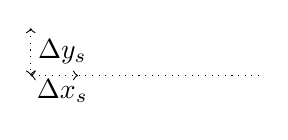
\begin{tikzpicture}
	\magnet {0} {0} {0}{}{1};
	\hall {3.0}{-0.6} {0};
	\draw[<->,dotted] (0,0)--(0,-0.6);
	\draw[<->,dotted] (0, -0.6)--(0.6,-0.6);
	\draw[dotted] (2.9,-0.6)--(0.6,-0.6);
	\node at (0.4,-0.3){$\Delta y_s$};
	\node at (0.4,-0.8){$\Delta x_s$};
	\end{tikzpicture}
	\caption{Shema definicije statične ekscentričnosti}
	\label{fig:def_sta_eks}
\end{figure}

%Po enakem razmišljanju kot v zgornjih poglavjih, sedaj zarotirajmo Hall-ovo sondo za kot \kol{-\theta} okoli izhodišča. Hall-ova sonda se giblje po krožnici z radijem $\sqrt{(x_0+\Delta x_s)^2+(y_0+\Delta y_s)^2}$.

%Statična ekscentričnost tako vpliva le na spremembo radija krožnice, ki jo opiše Hall-ova sonda ob rotaciji nad magnetom.

\begin{figure}[h!]
	\centering
	\begin{tikzpicture}
	\magnet {0} {0} {0}{}{1};
	\hall {1.69}{-1.67} {-30};
	\draw[<->,dotted] (0,0)--(-0.3,-0.52);
	\draw[dotted] (1.69,-1.67)--(-0.3,-0.52);
	\draw [dashed] (0,0) -- (2.377,0) arc(0:-30:2.377)--(0,0);
	\node at (0.8,-0.2) {\kol{-\theta}};
	\draw [dotted] (0,0)circle[radius=2.377];
%    \draw [dotted, <->] (0,0)--(2.06,1.19);
%    \node at (4.03,0.6){$\sqrt{(x_0+\Delta x_s)^2+(y_0+\Delta y_s)^2}$};
	\draw [dotted, <->] (0,0)--(1.69,-1.67);
    \draw [->] (1.5,0) arc (0:-30:1.5);
	\end{tikzpicture}
	\caption{Potek sonde ob vrtenju glede na magnet ob statični ekscentričnosti}
	\label{fig:def_sta_eks_stat}
\end{figure}



\begin{equation}
\label{equ:rotacija_hall_stat}
\begin{bmatrix} x\\y \end{bmatrix}=
\begin{bmatrix} \cos(\theta)&\sin(\theta)\\-\sin(\theta)&\cos(\theta) \end{bmatrix}
\begin{bmatrix} x_0+\Delta x_s\\y_0+\Delta y_s \end{bmatrix}
\end{equation}







\section{Končna enačba za določanje lokacije Hall-ove sonde}

%Do sedaj smo postopoma izpeljali enačbe za:
%\begin{itemize}
%  \item sistem magneta in Hall-ove sonde ob pravilni montaži
%  \item sistem magneta in Hall-ove sonde z dinamično ekscentričnostjo magneta
%  \item sistem magneta in Hall-ove sonde s statično ekscentričnostjo Hall-ove sonde
%\end{itemize}

(\ref{equ:rotacija_hall_din}) in (\ref{equ:rotacija_hall_simplify}) sta med seboj neodvisni zato se ju lahko združi.

\begin{equation}
\label{equ:rotacija_hall_koncna}
\begin{bmatrix} x\\y \end{bmatrix}=
\begin{bmatrix} \cos(\theta)&\sin(\theta)\\-\sin(\theta)&\cos(\theta) \end{bmatrix}
\begin{bmatrix} x_0+\Delta x_s\\y_0+\Delta y_s \end{bmatrix}-
\begin{bmatrix} \Delta x_d\\\Delta y_d \end{bmatrix}
\end{equation}


%Ogledali smo si, kako je ob rotaciji locirana Hall-ova sonda glede na magnet. Ogledali smo si tudi, kako na lokacijo sonde vplivati dinamična in statična ekscentričnost. S poznavanjem magnetnega polje $B_z=B_z(x , y)$, lahko določimo kakšno vrendost polja $B_z$ pomeri Hall-ova sonda ob rotaciji ($B_z=B_z(\theta)$). Ob poznavanju polja $B_z$, lahko določimo zasuk magneta glede na postavitev Hallove sonde.


\chapter{Izpeljava poteka polja $B_z(\theta)$ in ocena napake zaradi ekscentričnosti}

%V tem poglavju si bomo ogledali kakšno magnetno polje  pomeri Hall-ova sonda. Ogledali si bomo magnet, ter kako senzor RM44 meri magnetno polje. Preko pomirjenega polja, bomo izračunali kakšna je napake pomerjenega kota od referenčnega in kako se napaka spreminja z ekscentričnostjo.

\section{Definicija  gostote magnetnega polja $B_z$}

Predlagan magnet s strani proizvajalca senzorja je radialno magnetiziran s premerom 4 mm in višino 4 mm (slika \ref{magnet4mm}).
\begin{figure}[h]
	\centering
	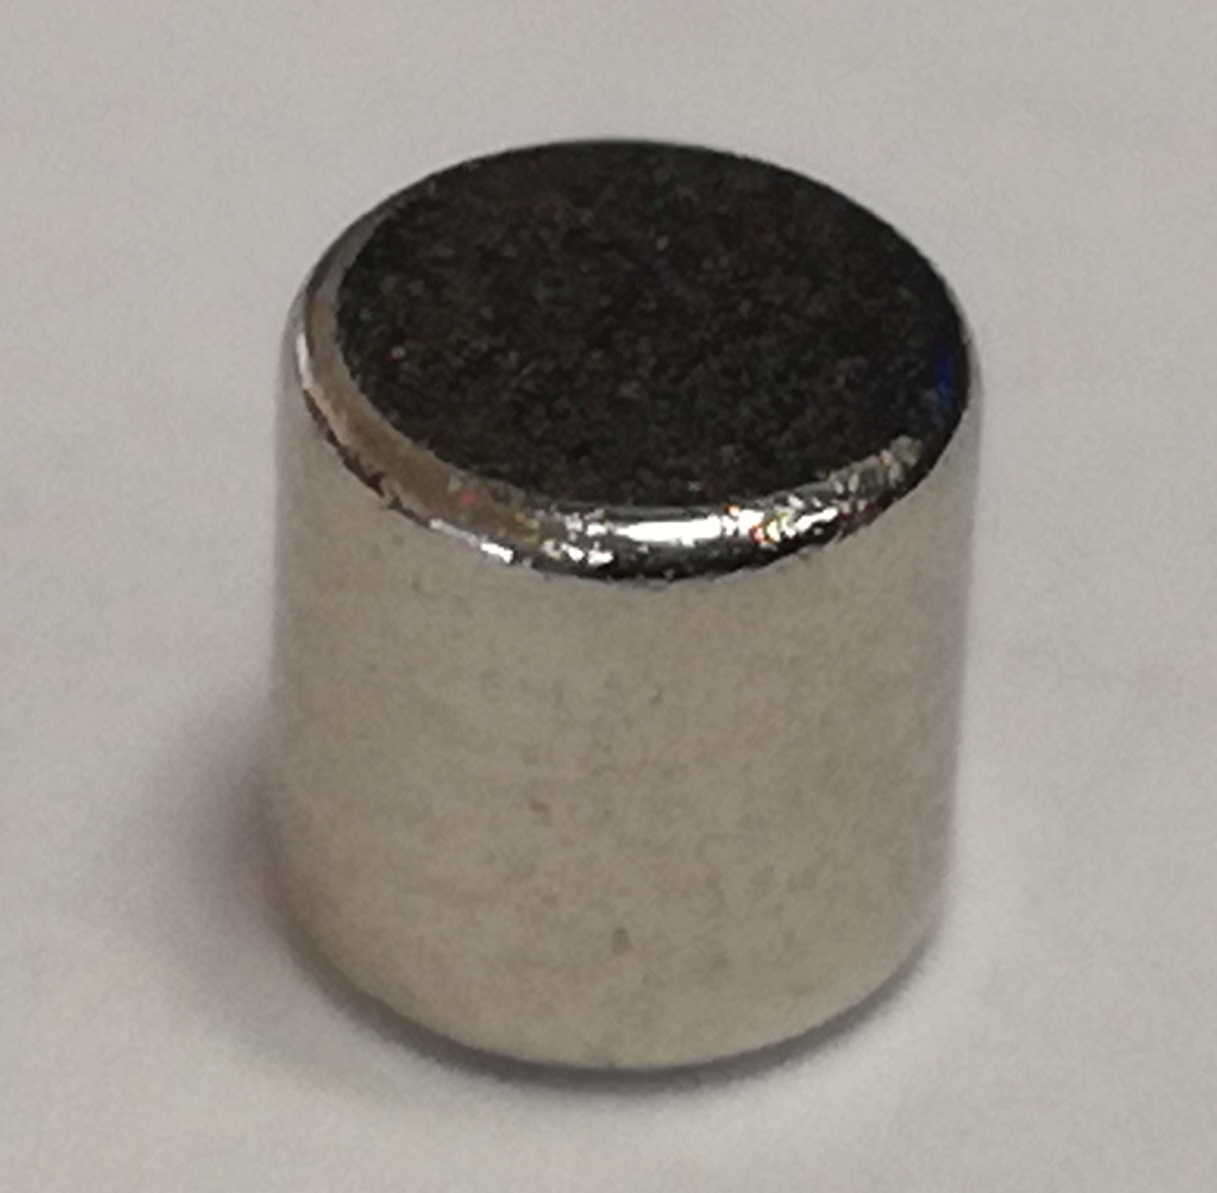
\includegraphics[width=0.75\columnwidth]{./Slike/magnet4mm.png}
	\caption{Primer magneta predlagan s strani proizvajalca RLS}
	\label{magnet4mm}
\end{figure}
Dajalnik pozicije RM44 meri z-komponento gostote magnetnega polja \cite{AM8192}. Potek komponente $B_z$ nad cilindričnim magnetom je prikazan na sliki \ref{fig:magnetno_polje}.

%Magsnetno polje  v prostoru lahko izračunamo z Biot-Savartovim zakonom. Poznati moramo specifikacije trajnega magneta in izračunati integral po prostoru. Tako dobimo v poljubni točki v prostoru vrednost B.  Hall-ove sonde v senzorju RM44 merijo le z-komponento magnetnega polja, zato se lahko osredotočimo le nanjo. Odvistnost z-komponente vektorja B na konstantni višini od magneta je vidno na sliki \ref{fig:magnetno_polje}.



\begin{figure}[h]
	\centering
		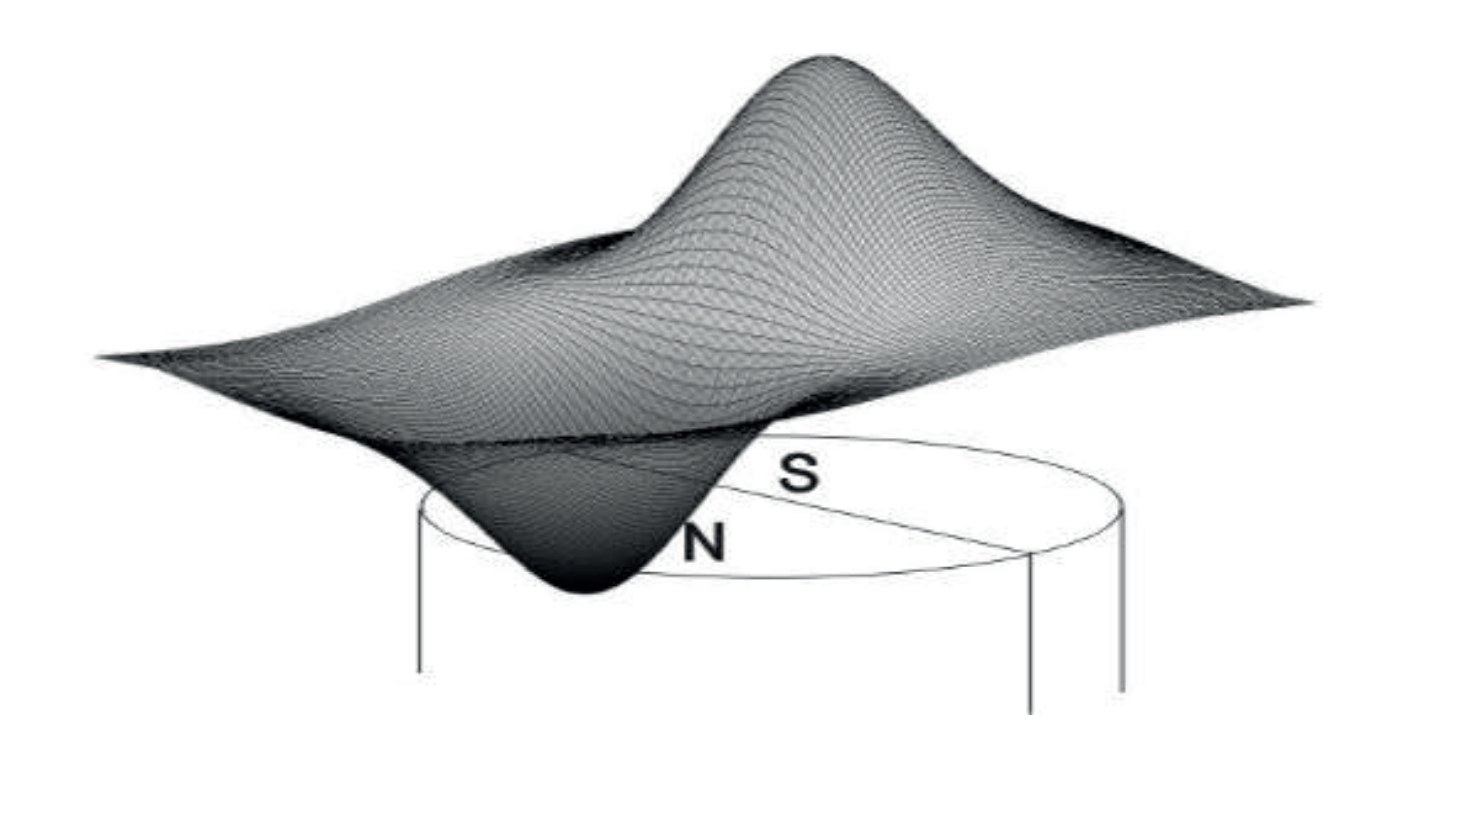
\includegraphics[width=0.75\columnwidth]{./Slike/magnetno_polje.jpg}
	\caption{z-komponenta vektorja gostote magnetnega polja nad cilindričnim magnetom \cite{AM8192}}
	\label{fig:magnetno_polje}
\end{figure}


Potek z-komponente se lahko izračuna po Biot-Savartovim zakonom oz. z numerično seštevanjem prispevke posameznih delčkov magneta. Za oceno napake, se magnetno polje z komponente v okolici osi vrtenja magneta aproksimira z ravnino (\ref{equ:poljeB}).

\begin{equation}
\label{equ:poljeB}
B_z(x,y)=k\cdot x.
\end{equation}

Aproksimacija zadostuje za oceno napake. S poznavanjem lokacije sonde glede na magnet, se lahko izračuna merjena komponenta magnetnega polja. Aprokisimirano polje je linearno odvisno od x komponente (\ref{equ:poljeB}). Za lažje razumevanje naj bo $k$ enak 1.

\section{Postavitev Hallovih sond in pomerjeno polje v odvistnosti od ekscentričnosti}
%Sedaj si oglejmo, kako bi določili kot zasuka poljubne točke okoli izhodišča. Definirajmo kartezični koordinatni sistem, in v njem poljubno točko $(x_0,y_0)$, ki ni v izhodišču(Slika \ref{fig:dolocitev_kota}).
%Za določanje kota $\varphi$ je potrebno poznati poznati položaj točke. Kot $\varphi$ določimo preko trigonometrične funkcije $\arctan$: $$\varphi=\arctan\frac{y_0}{x_0}$$
%
%
%
%\begin{figure}[h!]
%	\centering
%	\begin{tikzpicture}[scale=4]
%	\CaCS{0.75}{0}{0}
%	\draw [->,thick](0,0)--(-0.5,0.2855);
%	\draw (0.15,0) arc (0:150:0.15);
%	\node at (0.05,0.05){$\varphi$};
%%	\node at (-0.5,0.285) {\textbullet};
%	\node at (-0.32,0.35) {($x_0$,$y_0$)};
%	\end{tikzpicture}
%	\caption{Slika za pomoč pri določanju kota}
%	\label{fig:dolocitev_kota}
%\end{figure}
%
%
%Za določitev kota $\varphi$  je dovolj poznati že projekciji vektorja na koordinatni osi(slika \ref{fig:dolocitev_kota_2}),
%
%\begin{figure}[h!]
%	\centering
%	\begin{tikzpicture}[scale=4]
%	\CaCS{0.75}{0}{0}
%	\draw [->,thick](0,0)--(-0.5,0.2855);
%	\draw (0.15,0) arc (0:150:0.15);
%	\node at (0.05,0.05){$\varphi$};
%	\draw [dashed] (-0.5,0.2855)--(-0.5,0);
%	\draw [dashed] (-0.5,0.2855)--(0,0.2855);
%	%	\node at (-0.5,0.285) {\textbullet};
%%	\node at (-0.32,0.35) {($x_0$,$y_0$)};
%	\node at(-0.5,-0.1){$x_0$} ;
%	\node at(0.1,0.2855){$y_0$};
%	\end{tikzpicture}
%	\caption{Slika za pomoč pri določanju kota}
%	\label{fig:dolocitev_kota_2}
%\end{figure}
%
%
%če poznamo projekciji točke na koordinatni osi, je to zadosten pogoj za določitev kota $\varphi$.
%Projekcijo lahko pridobimo če opazujemo projekciji položaja točke v koordinatnih oseh.
%
%Sedaj si predstavljajmo da ta poljubna točka predstavlja enega od polov magneta. Za poznavanje zasuka pola magneta, je dovolj odčitanje polja na koordinatnih oseh. Hall-ovi sondi ne smeti biti postavljeni na isto koordinatno os. Ni nujno da sta sondi postavljeni pravokotno druga na drugo, si pa s tem prihranimo korak v katerem bi bilo potrebno izračunati projekcijo na pravokotni koordinatni osi.
%
%Iz zgornjega razmisleka lahko sedaj smiselno postavimo Hall-ovi sondi v koordinatni sistem. Najprimerneje ju je postaviti na koordinatni osi (Slika \ref{fig:zacetna_postavitev_sond}). Sondi postavimo na enako razdaljo od izhodišča $r_0$. Tako bo zajem poteka polja ob rotaciji magneta enak, le fazno zamaknjeno.


Za izračun kota je potrebno poznati polje v vsaj dveh točkah nad magnetom. Simulacijski model vsebuje 2 Hallovi sondi na koordinatnih oseh, oddaljeni od izhodišča za $r_0$.

\begin{figure}[h!]
	\centering
	\begin{tikzpicture}[scale=1]
	\CaCS{3}{0}{0}
	\senzorja{0}{0}{0}{}
%	\magnet {0} {0} {10}{ }{0}
	\node at (2.0,-0.5){$\mathrm{H}_1(r_0,0)$};
	\node at (-1,2.3){$\mathrm{H}_2(0, r_0)$};
	\end{tikzpicture}
	\caption{Začetna postavitev Hallovih sond}
	\label{fig:zacetna_postavitev_sond}
\end{figure}

S poznavanjem položaja sonde glede na magnet (\ref{equ:rotacija_hall_koncna}) in funkcije polja (\ref{equ:poljeB}) se lahko določi potek polja sonde. Sondi ob obratu vsaka pomeri svoje polje. Potek polja pomerjen s sondo v abcisni osi ($H_1$), je v idealni montaži podoben signalu kosinus, zato je poimenovan $cos$. Potek polja pomerjenega s sondo v ordinatni osi ($H_2$) je za $90^\circ$ zamaknjeno proti $cos$, zato je potek imenovan $sin$.

\begin{equation}\label{equ:Bx_splosna}
cos=B_{H_1}(\theta,r_0,\Delta x_s, \Delta y_s, \Delta x_d)= r_0 \cos\theta +\Delta x_s \cos\theta +\Delta y_s \sin\theta -\Delta x_d
\end{equation}
\begin{equation}\label{equ:By_splosna}
sin=B_{H_2}(\theta,r_0,\Delta x_s, \Delta y_s, \Delta x_d)= r_0 \sin\theta +\Delta x_s \cos\theta +\Delta y_s \sin\theta-\Delta x_d
\end{equation}

%Zajeta signala bom od tu naprej imenoval sinus ($sin$) in cosinu ($cos$), ker je to njuna osnovna oblika.
\subsection{Sprememba magnetnega polja zaradi ekscentričnosti}

%Oglejmo si primer kakšno polje zajameti Hall-ovi sondi, ko ekscentričnosti ni. $sin$ in $cos$ izraza se poenostavita in dobimo poteka v obliki sinusa ter kosinusa z enako amplitudo (Slika \ref{./Napake/sincos_00}).

%\slikaeps{Poteka $sin$ in $cos$ brez ekscentričnosti pri $r_0 = 1$ mm}{./Napake/sincos_00}
%\newpage
%Upoštevajmo sedaj le statični ekscentričnosti $\Delta x_s$ in $\Delta y_s$. $\Delta x_d$ postavimo na 0.   Enačbi (\ref{equ:Bx_splosna}) in (\ref{equ:By_splosna}) lahko preuredimo v izraza:

Iz izrazov (\ref{equ:Bx_splosna}) in (\ref{equ:Bx_splosna}) brez upoštevanja ekscentričnosti sta $sin$ in $cos$ enake amplitude ter fazno zamaknjena za $90^\circ$. Z upoštevanjem statične ekscentričnosti se med $sin$ in $cos$ zmanjša fazni kot ter spremni amplituda (\ref{equ:Bx_stat}) (\ref{equ:By_stat}). Ob dinamični ekscentričnosti signala pridobita enosmerni komponenti (\ref{equ:Bx_din}) (\ref{equ:By_din}).


\begin{equation}
\label{equ:Bx_stat}
cos(\theta,r_0,\Delta x_s, \Delta y_s)= \sqrt{(r_0+\Delta x_s)^2+\Delta y_s^2}\cos(\theta -\arctan \frac{\Delta y_s}{r_0+\Delta x_s})
\end{equation}
\begin{equation}\label{equ:By_stat}
sin(\theta,r_0,\Delta x_s, \Delta y_s)= \sqrt{\Delta x_s^2+(r_0+\Delta y_s)^2} \sin(\theta +\arctan \frac{\Delta x_s}{r_0+\Delta y_s})
\end{equation}

%Iz njiju vidimo spremenjena poteka. Signaloma se je spremenila amplituda in fazni zamik (Slika \ref{./Napake/sincos_xs}).

%\slikaeps{Poteka $sin$ in $cos$ pri $r_0 = 1$ mm in upoštevanjem 0,1 mm statični ekscentričnosti v x-osi }{./Napake/sincos_xs}
%\newpage
%Postavimo sedaj vrednosti $\Delta x_s$ in $\Delta_ys$ na 0, $\Delta x_d$ predpostavimo da ni 0.
\begin{equation}
\label{equ:Bx_din}
cos(\theta,r_0,\Delta x_s, \Delta y_s, \Delta x_d)= r_0 \cos\theta-\Delta x_d
\end{equation}
\begin{equation}
\label{equ:By_din}
sin(\theta,r_0,\Delta x_s, \Delta y_s, \Delta x_d)= r_0 \sin\theta-\Delta x_d
\end{equation}
%Polji obdržita enako amplitudo ter fazo, vendar dobita enosmerno komponento (Slika \ref{./Napake/sincos_xd}).
%\slikaeps{Poteka $sin$ in $cos$ pri $r_0 = 1$ mm in upoštevanjem 0,1 dinamične ekscentričnosti v x-osi}{./Napake/sincos_xd}\newpage
\section{Premik senzorja v z smeri}

%Poglejmo si še kako vpliva sprememba premikanja senzorja v z smeri.
Pri magnetnem polju aprokismiranem z ravnino (\ref{equ:lin_polje}), se gostota magnetnega polja pri obeh sondah spreminja enako. To se v enačbah odraža le kot dodaten faktor. Upoštevano spremembo polja zaradi premika senzorja po z osi se izrazi kot:
\begin{equation}\label{equ:Bx_z}
cos=k_z( r_0 \cos\theta +\Delta x_s \cos\theta +\Delta y_s \sin\theta -\Delta x_d)
\end{equation}
\begin{equation}\label{equ:By_z}
sin=k_z( r_0 \sin\theta +\Delta x_s \cos\theta +\Delta y_s \sin\theta-\Delta x_d)
\end{equation}

Z vstavitvijo formul v $\arctan$ se faktor $k_z$ nahaj tako v števcu kot imenovalcu ter se okrajša. Ti poteki polj veljajo le z upoštevanjem aprokismiranega polja (\ref{equ:poljeB}).



\chapter{Potek napake funkcije atan2 ob popačenju vhodnih signalov}
Izhod enkoderja je podatek o zasuku. Iz pomerjenega polja, sledi izračun kota preko inverza funkcije tangens.
% preko funkcija $\arctan$\cite{Matematika1}. V programskem poaketu MATLAB se za izračun inverzne funkcije tangens na območju 4 kvadrantov uporalblja funkcija atan2d()\cite{atan2dMatlab}.
%Da si lažje predstavljamo, kako se bo napaka odražala v obliki digitalnega izhoda, si oglejmo posamezno deformacijo signalov sinus in cosinus. Deformacija sinusa in cosinusa zaradi nepravilne montaže, vpliva le na enosmerno komponento, amplitudo in fazni kot med signaloma.
%Ogledali si bomo kako vplivajo na izračunan kot, različne amplitude signalov sinus in cosinus, neortogonalost oz. fazni zamik sinusa in kosinusa različen od $90^\circ$. Ogledali si bomo tudi pojav enosmernih komponenet v sinusu in cosinusu, in za konec še vpliv višjih harmonikov, ki niso posledica nepravilne montaže, vendar je prav da jih omenim.
V programu MATLAB se za izračun kota uporablja funkcijo atan2(); za izhodno vrednost kota v radianih oz. atan2d(); za vrednost v stopinjah \cite{atan2Matlab}\cite{atan2dMatlab}. Različne literature \cite{Napaka_osnova} opisujejo napake zaradi popačitve signalov $sin$ $cos$. Napaka je izražena v obliki enosmerne komponente ter prvega oz drugega harmonika, kateri od primera do primera najbolj izstopa. V nadaljevanju je prikazano, kako popačen signal kot vhod v funkcijo atan2d(); vpliva na napako ter kako se odraža tudi na višjih harmonikih. Za majhne popačenja signalov, literatura nakazuje linearno naraščanje napake.

%Na tej točki je prav da definiram še napako pomejrenega kota $\varepsilon$, ki predstavlja razliko med merjenim in referenčnim kotom.

%\begin{equation}
%\varepsilon = \varphi - \mathrm{atan2}(\sin{\theta},\cos{\theta})
%\end{equation}


\section{Različne amplitude}

Vhodna signala v atan2d();, sta:
\begin{eqnarray}
\label{equ:def_sin_ama}
&Sin = k \sin(\theta)\\
\label{equ:def_cos_amp}
&Cos =\cos(\theta)
\end{eqnarray}

limita ko gre k proti neskončnost:
\begin{equation}
\lim_{k \rightarrow \infty} \mathrm{atan2}(k \sin{\theta},\cos{\theta})
\end{equation}

\slikaeps{$\varepsilon$ ob limiti k v neskončnost }{./Napake/k_lim}

Kot $\varepsilon$, se bo ob limiti  izrazila v obliki , ki jo lahko izrazimo z Fourierovo vrsto \cite{fourierova_vrsta}:

\begin{equation}
\varepsilon = \frac{180}{\pi}\sum_{n=1}^{\infty}\frac{1}{n} \sin 2 n \theta
\end{equation}

V napaki nastopajo le sodi harmoniki. S opazovanjem sodih harmonikov napake pri različnih k-jih in uporabo funkcije Curve Fitting tool \cite{cftool}, sem določil fukcijo poteka napake v odvistnosti od k. 

\begin{equation}
\label{vrsta_k}
\varepsilon_p =\frac{180}{\pi}\sum_{n=1}^{\infty}\frac{1}{n}(\frac{k-1}{k+1})^n \sin 2 n \theta
\end{equation}

\slikaeps{$\varepsilon$ pri k=1.1 }{./Napake/napaka_amp11}
\slikaeps{Razlika med napako izračunano s funkcijo atan2 in izračnunano napako z vrsto (prvih 15 členov) po (\ref{vrsta_k}) pri k= 1.1 }{./Napake/razlika_amp11}


\newpage


\section{Različne enosmerne komponente}

Enosmerna komponenta se lahko pojavi tako v $sin$, $cos$ ali v obeh.

Vhodna signala v atan2d();, sta:
\begin{eqnarray}
\label{equ:def_sin_ama}
&Sin = \sin(\theta) + B_0\\
\label{equ:def_cos_amp}
&Cos =\cos(\theta) +A_0
\end{eqnarray}

V podpoglavjih so obrvnavani različni primeri enosmernih komponent v signalih $sin$ in $cos$.
\subsection{Enosmerna komponenta le v signalu $sin$}

Z limito $B_0$ v neskončnost, in izpeljavi napake v obliko Fourierove vrste, se napaka izrazi kot:

\slikaeps{$\varepsilon$ ob limiti $B_0$ v neskončnost }{./Napake/lim_sin}

\begin{equation}
\varepsilon = \frac{180}{\pi}\sum_{n=1}^{\infty}\frac{2}{n} \sin (n \theta + 90 n)
\end{equation}


Z analizo potekov posameznega harmonika napake in uporabe Curve Fitting tool je bila najdena funkcija, ki opiše odvisnost napake od enosmerne komponente v signalu $sin$.

\begin{equation}
\label{vrsta_sinoff}
\varepsilon_p=
\begin{cases}
\frac{180}{\pi}\sum_{n=1}^{\infty}\frac{2-|B_0|^{-n}}{n} \sin (n \theta -  90 n), & B_0\leq -1 \\
\frac{180}{\pi}\sum_{n=1}^{\infty}\frac{B_0^n}{n} \sin (n \theta + 90 n), & |B_0|\leq 1 \\
\frac{180}{\pi}\sum_{n=1}^{\infty}\frac{2-B_0^{-n}}{n} \sin (n \theta + 90 n), & B_0\geq 1
\end{cases}
\end{equation}

\slikaeps{$\varepsilon$ pri $B_0=$ 0,1 }{./Napake/napaka_sin01}
\slikaeps{Razlika med napako izračunano s funkcijo atan2d in napako izračunano z (\ref{vrsta_sinoff}) pri $B_0=$ 0,1 in $n < 20$}{./Napake/razlika_sin01}




\subsection{Enosmerna komponenta signala $cos$}

Postopek je ponovljen tudi za enosmerno komponento v signalu $cos$


\begin{equation}
\lim_{a_0 \rightarrow \infty} \mathrm{atan2}(\sin{\theta},\cos{\theta} + A_0)
\end{equation}
\slikaeps{$\varepsilon$ ob limiti $A_0$ v neskončnost }{./Napake/lim_cos}

Napaka (slika \ref{./Napake/lim_cos}) je proti napaki na  sliki \ref{./Napake/lim_sin} le fazno zamaknjena.
To se izrazi tudi v Fourierovi vrsti.
\begin{equation}
\varepsilon = \frac{180}{\pi}\sum_{n=1}^{\infty}\frac{2}{n} \sin (n \theta+ 90 n)
\end{equation}

Potek napake v odvisnosti od $A_0$ je (\ref{vrsta_cosoff})

\begin{equation}
\label{vrsta_cosoff}
\varepsilon_p=
\begin{cases}
\frac{180}{\pi}\sum_{n=1}^{\infty}(-1)^n\frac{2-|A_0|^{-n}}{n} \sin (n \theta ), & A_0\leq -1 \\
\frac{180}{\pi}\sum_{n=1}^{\infty}(-1)^n\frac{A_0^n}{n} \sin (n \theta ), & |A_0|\leq 1 \\
\frac{180}{\pi}\sum_{n=1}^{\infty}(-1)^n\frac{2-A_0^{-n}}{n} \sin (n \theta ), & A_0\geq 1
\end{cases}
\end{equation}

\slikaeps{$\varepsilon$ pri $A_0=$ 0,1 }{./Napake/napaka_cos01}
\slikaeps{Razlika med napako izračunano s funkcijo atan2d in napako izračunano z (\ref{vrsta_sinoff}) pri $A_0=$ 0,1 in $n < 20$}{./Napake/razlika_cos01}

\newpage
\subsection{Enosmerna komponenta pri obeh signalih}
\label{2_offseta}
Enosmerna komponenta pri obeh signalih je označena z $C_0$.
%\begin{equation}
%\varphi = \mathrm{atan2}(\sin{\theta} + c_0,\cos{\theta} + c_0)
%\end{equation}

Limita napake ko gre $C?0$ proti neskončnosti se v Fourierovi vrsti izrazi kot:

%\begin{equation}
%\lim_{c_0 \rightarrow \infty} \mathrm{atan2}(\sin{\theta} + c_0,\cos{\theta}+ c_0) 
%\end{equation}

\slikaeps{$\varepsilon$ ob limiti $c_0$ v neskončnost }{./Napake/lim_sincos}


\begin{equation}
\varepsilon = \frac{180}{\pi}\sum_{n=1}^{\infty}\frac{2}{n} \sin (n \theta- 90 n)
\end{equation}


Odvisnost napake ob spreminjanju enosmernih komponent pri obeh signalih se je izrazilo v (\ref{vrsta_sincosoff}).


\begin{equation}
\label{vrsta_sincosoff}
\varepsilon_p=
\begin{cases}
\frac{180}{\pi}\sum_{n=1}^{\infty}\frac{2-|\sqrt{2}c_0|^{-n}}{n} \sin (n \theta + 90 n), & c_0\leq -\frac{\sqrt{2}}{2} \\
\frac{180}{\pi}\sum_{n=1}^{\infty}\frac{(\sqrt{2}c_0)^n}{n} \sin (n \theta - 90 n), & |c_0|\leq \frac{\sqrt{2}}{2} \\
\frac{180}{\pi}\sum_{n=1}^{\infty}\frac{2-(\sqrt{2}c_0)^{-n}}{n} \sin (n \theta - 90 n), & c_0\geq \frac{\sqrt{2}}{2}
\end{cases}
\end{equation}

\slikaeps{$\varepsilon$ pri $C_0=$ 0,1 }{./Napake/napaka_sincos01}
\slikaeps{Razlika med napako izračunano s funkcijo atan2d in napako izračunano z (\ref{vrsta_sincosoff}) pri $C_0=$ 0,1 in $n < 20$}{./Napake/razlika_sincos01}




\section{Neorotogonalnost signalov}

Napaka se pojavi tudi, če signala $sin$ in $cos$ nista fazno zamaknjena za točno $90^\circ$.
Vhodna signala imata obliko:
\begin{eqnarray}
\label{equ:def_sin_fis}
&Sin = \sin(\theta + \varphi_{s})\\
\label{equ:def_cos_fis}
&Cos =\cos(\theta+\varphi_{c})
\end{eqnarray}

Napako se določi posamično za vsakega od parametrov. Drugi je takrat enak 0. Na koncu se enačbi združi. Za določanje limite ni potrebno iti proti neskončnosti, ampak le do najslabše možnosti, ki je pri $\pm 90^\circ$:
\begin{equation}
\label{equ:fis_lim}
\varepsilon = \lim_{\varphi_{s} \rightarrow 90^\circ} \mathrm{atan2}(Sin ,Cos)- \mathrm{atan2d}(\sin(\theta),\cos(\theta))
\end{equation}
Potek napake $\varepsilon$ s slike \ref{fig:lim_sin_fis} predstavi vrsta (\ref{equ:lim_fis_vrsta}).
\slikaeps{Napaka $\varepsilon$ ob limiti $\varphi_{s} \rightarrow 90^\circ$}{./Napake/lim_sinfaza}

\begin{equation}
\label{equ:lim_fis_vrsta}
\varepsilon = 45^\circ - \frac{180}{\pi}\sum_{n=1}^{\infty}\frac{1}{n} \sin (2n \theta)
\end{equation} 
Iz  izraza je vidno nastopanje enosmerne komponente in sodih harmonikov. Z opazovanjem sodih harmonikov napake pri različnih faznih kotih je bil dobljen izraz napake v odvistnosti od faznih zamikov $sin$ in $cos$ na idealna signala.

\begin{multline}
\label{equ:fis_err}
\varepsilon(\varphi_{s},\varphi_{c}) = \frac{\varphi_{s}+\varphi_{c}}{2}+\\ \frac{180}{\pi}\sum_{n=1}^{\infty}\frac{1}{n} (\mathrm{tan}\frac{\varphi_{s}-\varphi_{c}}{2})^n \sin (2n \theta+n(90^\circ +\varphi_{s}+\varphi_{c}))
\end{multline}


\newpage
\section{Potek napake pri statični ekscentričnosti v smeri x}

Statična ekscentričnost povzroči v $sin$ in $cos$ razliko amplitud kot spremembo faz. Za vsako ekscentričnost posebaj je bil izračunan potek napake aproksimirn z racionalno funkcijo.

Definirana vhodna signala:
\begin{eqnarray}
\label{xs_analit}
sin = r_0 \sin(\theta) + \Delta x_s \cos(\theta) \\
cos = r_0 \cos(\theta) + \Delta x_s \cos(\theta)
\end{eqnarray}

Opravljena je bila limita $\Delta x_s$ v neskončnost. V napaki nastopa enosmerna komponenta in sodi harmoniki. Funkcija ki predstavlja odvisnost napake od statične ekscentričnosti je (\ref{vrsta:xs}).

 \begin{equation}
 \label{vrsta:xs}
 \varepsilon_p = \mathrm{atan}\frac{\Delta x _s}{\Delta x _s+2r_0}+\frac{180}{\pi} \sum_{n=1}^{\infty}\frac{1}{n} (\frac{\Delta x _s}{\sqrt{\Delta x _s^2+2 r_0 \Delta x _s+2r_0^2}})^n \sin (2n \theta+n (90+ \mathrm{ atan}(\frac{\Delta x _s+r_0}{r_0})))
 \end{equation}
 
 Pri čemer:
 $$\Delta x_s > -r_0$$

 \section{Potek napake pri statični ekscentričnosti v smeri y}
 
 Postopek ponovljen za  ekscentričnost v y smeri. Pričakovan je podoben potek kot pri ekscentričnosti v x smeri.
 
Izračunana vrsta napake v odvisnosti od  $\Delta y_s$ je:
 
  \begin{equation}
   \label{vrsta:ys}
 \varepsilon_p = \mathrm{atan}\frac{-\Delta y _s}{\Delta y _s+2r_0}+\frac{180}{\pi} \sum_{n=1}^{\infty}\frac{1}{n} (\frac{\Delta y _s}{\sqrt{\Delta y _s^2+2 r_0 \Delta y _s+2r_0^2}})^n \sin (2n \theta+n (90+ \mathrm{ atan}(\frac{\Delta y _s+r_0}{r_0})))
 \end{equation}

 Pri čemer:
$$\Delta y_s > -r_0$$

\section{Potek napake pri dinamični ekscentričnosti v smeri x}

$sin$ in $cos$ se pri dinamični ekscentričnosti spreminjata, kot je bilo opisano pri napaki z enakima enosmernima komponentama. Rezultat napake v odvisnosti od dinamične ekscentričnosti je:


%Analogna signala se izrazita z naslednjim potekom:
%
%\begin{eqnarray}
%sin = r_0 \sin(\theta) - \Delta x_d \\
%cos = r_0 \cos(\theta) - \Delta x_d
%\end{eqnarray}
%
%Signala nas spomnita na poteka, ki smo ju obravnavali že v poglavju \ref{2_offseta}, zato bom tu napisal le rezultat. Razlikuje se le v predznaku.
%
\begin{equation}
\label{vrsta_xd}
\varepsilon_p=
\frac{180}{\pi}\sum_{n=1}^{\infty}\frac{1}{n}( \frac{-\sqrt{2}}{r_0}\Delta x_d)^n \sin (n \theta -  90 n)
\end{equation}

Pri čemer velja
$$|\Delta x_d|\leq \frac{r_0}{\sqrt{2}}$$
%
%
%V tem poglavju smo pogledali, poteke napake ob deformaciji analognih signalov. Ogledali smo si tudi, kako se bo napaka izrazila ob ekcentričnosti senzorja ter magneta. 
Za majhne odmike, je dovolj upoštevanje le prvega člena vrste, pri katerih se tudi predpostavi linearno naraščanje napake. V nadaljevanju bodo velikosti harmonikov v odvistnosti od povzročene ekscentričnosti aproksimirani s kubičnim polinomi. Da bo primerjava možna bodo poteki izračunani v tem poglavju razviti v Taylorjevo vrsto do tretje stopnje.
%, ter jih primerjal z izpeljavo v tem poglavju. Harmoniki katerih potek je npr racionalna funkcija (primer (\ref{vrsta:xs})), bom razvil v Taylorjevo vrsto do tretje stopnje, katero bom lahko primerjal s kubičnimi polinomi.
% 









%\section{Analitičen potek napake posamezne ekscentričnosti}
%
%S poznavanjem potekov polja posamezne sonde sedaj s funkcijo $\arctan$ izračunamo kot.
%
%\begin{equation}
%\label{equ:izracun_kota_splosna}
%\varphi(\theta,\Delta x_s, \Delta y_s, \Delta x_d)=\arctan\frac{B_y}{B_x}=\arctan\frac{r_0 \sin\theta +\Delta x_s \cos\theta +\Delta y_s \sin\theta-\Delta x_d}{r_0 \cos\theta +\Delta x_s \cos\theta +\Delta y_s \sin\theta -\Delta x_d}
%\end{equation}
%
%
%
%
%Iz podanega izraza (\ref{equ:izracun_kota_splosna}) je težko sklepati, kakšen bo potek pomerjenega kota.
%Na tem mestu definirajmo napako merjenega kota:
%\begin{equation}
%\varepsilon=\varphi-\theta
%\end{equation}
%
%Poglejmo si analitičen potek napake.  S spodaj opisanim postopkom se bomo izognili numeričnemu računanju funkcije $\arctan$.
%
%Signala $sin$ in $cos$ imata periodo $360^\circ$. Iz tega sledi, da bo tudi $\varepsilon$ imel periodo $360^\circ $. Pričakujem, da bo potek napake $\varepsilon$ v obliki :
%\begin{equation}
%\label{equ:nastavek}
%\varepsilon=A_0+A_1 \cos \theta +B_1 \sin \theta+A_2 \cos 2\theta +B_2 \sin 2\theta
%\end{equation}
%Tak nastavek sem vzel zaradi predvidene napake v podatkovnih listih citeAM8192.
%Za približek napake izraz  (\ref{equ:izracun_kota_splosna}) razvijmo v Taylorjevo vrsto po kotu $\theta$. V Taylorjevo vrsto razvjemo tudi nastavek pričakovanega poteka. Zaradi aproksimacije poteka merjenega kota se zadovoljimo z razvojem do petega reda. Za poenostavitev se bom ekscentričnosti lotil posamezno. V naslednjih podpoglavjih bom prikazal analitične rezultate posameznega harmonika. Izpeljavo bom le teoretično opisal.
%
%Oba izraza (\ref{equ:izracun_kota_splosna} in \ref{equ:nastavek} )razvijem do petega reda Taylorjeve vrste  po kotu $\theta$. Z združitvijo posameznih potenc $\theta$, pridobimo sistem petih enčb s petimi neznankami. S tem pridobim neznane faktorje $A_0$, $A_1$, $A_2$, $B_1$ in $B_2$. S poznavanjem teh faktorjev lahko ocenimo kaškni bodo poteki posameznih harmonikov, ob posameznih ekscentričnostih. Te rezultate Taylorjeve vrste lahko upoštevam le v okolici ničle. Izrazi so izpeljani za statični ekscentričnosti ter dinamično ekscentričnost v smeri x. Potekov dinamične ekscentričnosti v smeri y ni, saj ta ne nastopa v izrazu (\ref{equ:izracun_kota_splosna}).
%\subsection{Aproksimacija pomerjenega kota ob statični ekscentričnosti x}
%V izrazu (\ref{equ:izracun_kota_splosna}) upoštevamo le statično ekscentričnost $\Delta x_s$.
%\begin{equation}
%\label{equ:izracun_kota_xs}
%\varphi=\arctan \frac{r_0 \sin\theta +\Delta x_s \cos\theta}{r_0 \cos\theta +\Delta x_s \cos\theta}
%\end{equation}
%Z aproksimacijo po izrazu (\ref{equ:nastavek}) pridobimo koeficiente posameznega harmonika
%
%\begin{eqnarray}
%&A_0=\frac{-90 r_0^2  \Delta y_s (r_0^5+29 r_0^4 \Delta y_s+132 r_0^3  \Delta y_s^2+208 r_0 ^2  \Delta y_s^3+156 r_0  \Delta y_s^4+52 \Delta y_s^5)}{\pi (r_0^2+2 r_0 \Delta y_s+2 \Delta y_s^2)^4}+\arctan \frac{ \Delta y_s}{r_0+ \Delta y_s}\\
%&A_1=\frac{2280 r_0^2  \Delta y_s^2(r_0^4+5 r_0^3  \Delta y_s+8 r_0^2  \Delta y_s^2+6 r_0  \Delta y_s^3+2 \Delta y_s^4)}{\pi(r_0^2+2 r_0 \Delta y_s+2 \Delta y_s^2)^4}\\
%&B_1=-\frac{240 \Delta y_s^3(7r_0^3+18 r_0^2  \Delta y_s+18 r_0^2  \Delta y_s+18 r_0  \Delta y_s^2+8 \Delta y_s^3)}{\pi(r_0^2+2 r_0 \Delta y_s+2 \Delta y_s^2)^3}\\
%&A_2=\frac{90 r_0^2  \Delta y_s (r_0^5-3 r_0^4 \Delta y_s-28 r_0^3  \Delta y_s^2-48r_0 ^2  \Delta y_s^3-36 r_0  \Delta y_s^4-12 \Delta y_s^5)}{\pi(r_0^2+2 r_0 \Delta y_s+2 \Delta y_s^2)^4}\\
%&B_2=\frac{30 \Delta y_s (-3r_0^5-18 r_0^4 \Delta y_s-20 r_0^3  \Delta y_s^2 +12 r_0  \Delta y_s^4+8 \Delta y_s^5)}{\pi(r_0^2+2 r_0 \Delta y_s+2 \Delta y_s^2)^3}\\
%\end{eqnarray}
%Oglejmo si sliko potekov posameznih harmonikov.
%\slikaeps{Poteki amplitud prvega in drugega harmonika ter enosmerne komponente ob spreminjanju statične ekscentričnosti v x-osi}{potek_analitika_xs}
%Iz rezultatov lahko pričakujemo naraščanje drugega harmonika ter naraščanje enosmerne komponete.
%\subsection{Aproksimacija pomerjenega kota ob statični ekscentričnosti y}
%V izrazu (\ref{equ:izracun_kota_splosna}) upoštevamo le statično ekscentričnost $\Delta y_s$.
%\begin{equation}
%\label{equ:izracun_kota_ys}
%\varphi=\arctan \frac{r_0 \sin\theta +\Delta y_s \sin\theta}{r_0 \cos\theta +\Delta y_s \sin\theta}
%\end{equation}
%Z aproksimacijo po izrazu (\ref{equ:nastavek}) pridobimo koeficiente posameznega harmonika
%\begin{eqnarray}
%&A_0=\frac{-90 y_s (r_0^2-23r_0 y_s-24y _s^2)}{\pi r_0^3}\\
%&A_1=\frac{-1690 y_s^2(r_0+y_s)}{\pi r_0^3}\\
%&A_2=\frac{90 y_s(r_0^2+9r_0y_s+8y_s^2)}{\pi r_0^3}\\
%&B_1=\frac{240 y_s^3}{\pi r_0^3}\\
%&B_2=\frac{30 (3 r_0^2y_s-4 y_s^3)}{\pi r_0^3}
%\end{eqnarray}
%Oglejmo si sliko potekov posameznih harmonikov.
%\slikaeps{Poteki amplitud prvega in drugega harmonika ter enosmerne komponente ob spreminjanju statične ekscentričnosti v y-osi}{potek_analitika_ys}
%Iz grafa je razvidno, da do enosmerna komponenta upadala, drugi harmonik bo najbolj izrazit.
%\subsection{Aproksimacija pomerjenega kota ob dinamični ekscentričnosti x}
%Izraz  (\ref{equ:izracun_kota_splosna}) kjer upoštevamo le dinamično ekscentričnost se poenostavi v:
%\begin{eqnarray}
%&A_0=\frac{180(r_0 \Delta x_d(r_0^6-7r_0^5 \Delta x_d+18r_0^4 \Delta x_d^2-36r_0^2 \Delta x_d^4 +28r_0 \Delta x_d^5-8 \Delta x_d^6))}{\pi(r_0^2-2r_0 \Delta x_d+2 \Delta x_d^2)^4}-\arctan \frac{\Delta x_d}{r_0- \Delta x_d}\\
%&A_1=\frac{-180(r_0 \Delta x_d(r_0^6-8r_0^5 \Delta x_d+22r_0^4 \Delta x_d^2-44r_0^2 \Delta x_d^4 
%	+32r_0 \Delta x_d^5-8 \Delta x_d^6)}{\pi (r_0^2-2r_0 \Delta x_d+2 \Delta x_d^2)^4)}\\
%&A_2=\frac{-180(r_0^2 \Delta x_d^2 (r_0^4-4 r_0^3  \Delta x_d+8 r_0  \Delta x_d^3-4 
%	\Delta x_d^4)}{\pi (r_0^2-2 r_0  \Delta x_d+2  \Delta x_d^2)^4)}\\
%&B_1=\frac{60( \Delta x_d (3 r_0^5-18 r_0^4  \Delta x_d+64 r_0^3  \Delta x_d^2 -108 
%	r_0^2  \Delta x_d^3+84 r_0  \Delta x_d^4-32  \Delta x_d^5))}{\pi (r_0^2-2 r_0 
%	\Delta x_d+2  \Delta x_d^2)^3}\\
%&B_2=\frac{60 (2  \Delta x_d^3 (-4 r_0^3+9 r_0^2  \Delta x_d-6 r_0  \Delta x_d^2+2  \Delta x_d
%	^3))}{\pi(r_0^2-2 r_0  \Delta x_d+2  \Delta x_d^2)^3}
%\end{eqnarray}
%\slikaeps{Poteki amplitud prvega in drugega harmonika ter enosmerne komponente ob spreminjanju dinamične ekscentričnosti v x-osi}{potek_analitika_xd}
%S slike \ref{potek_analitika_xd} vidimo da bo izrazit le prvi harmonik, ki pri majhnih odmikih narašča linearno, kar je pričakovano po citeAM8192. 
%
%V tem poglavju smo si ogledali kakšno magnetno polje ustvari magnet in kako ga Hall-ove sonde zaznavajo. magnetno polje smo aproksimirali z ravnino in si ogledali poteke napake.  Spoznali smo tudi kako se bo izražala napaka pri posamezni ekscentričnosti.
%
%
%
%
%
%
%
%
%











